\chapter{Results and Discussion}

\section{Qualitative differences in film structure}

Three sets of thin films have been fabricated from three varying successive ionic layer adhesion and reaction processes.
Shown in Figure 3 are some of the images that were captured using the high power objective lens of a digital compound microscope.

\begin{figure}
  \centering
  \begin{subfigure}{.4\textwidth}
    \centering
    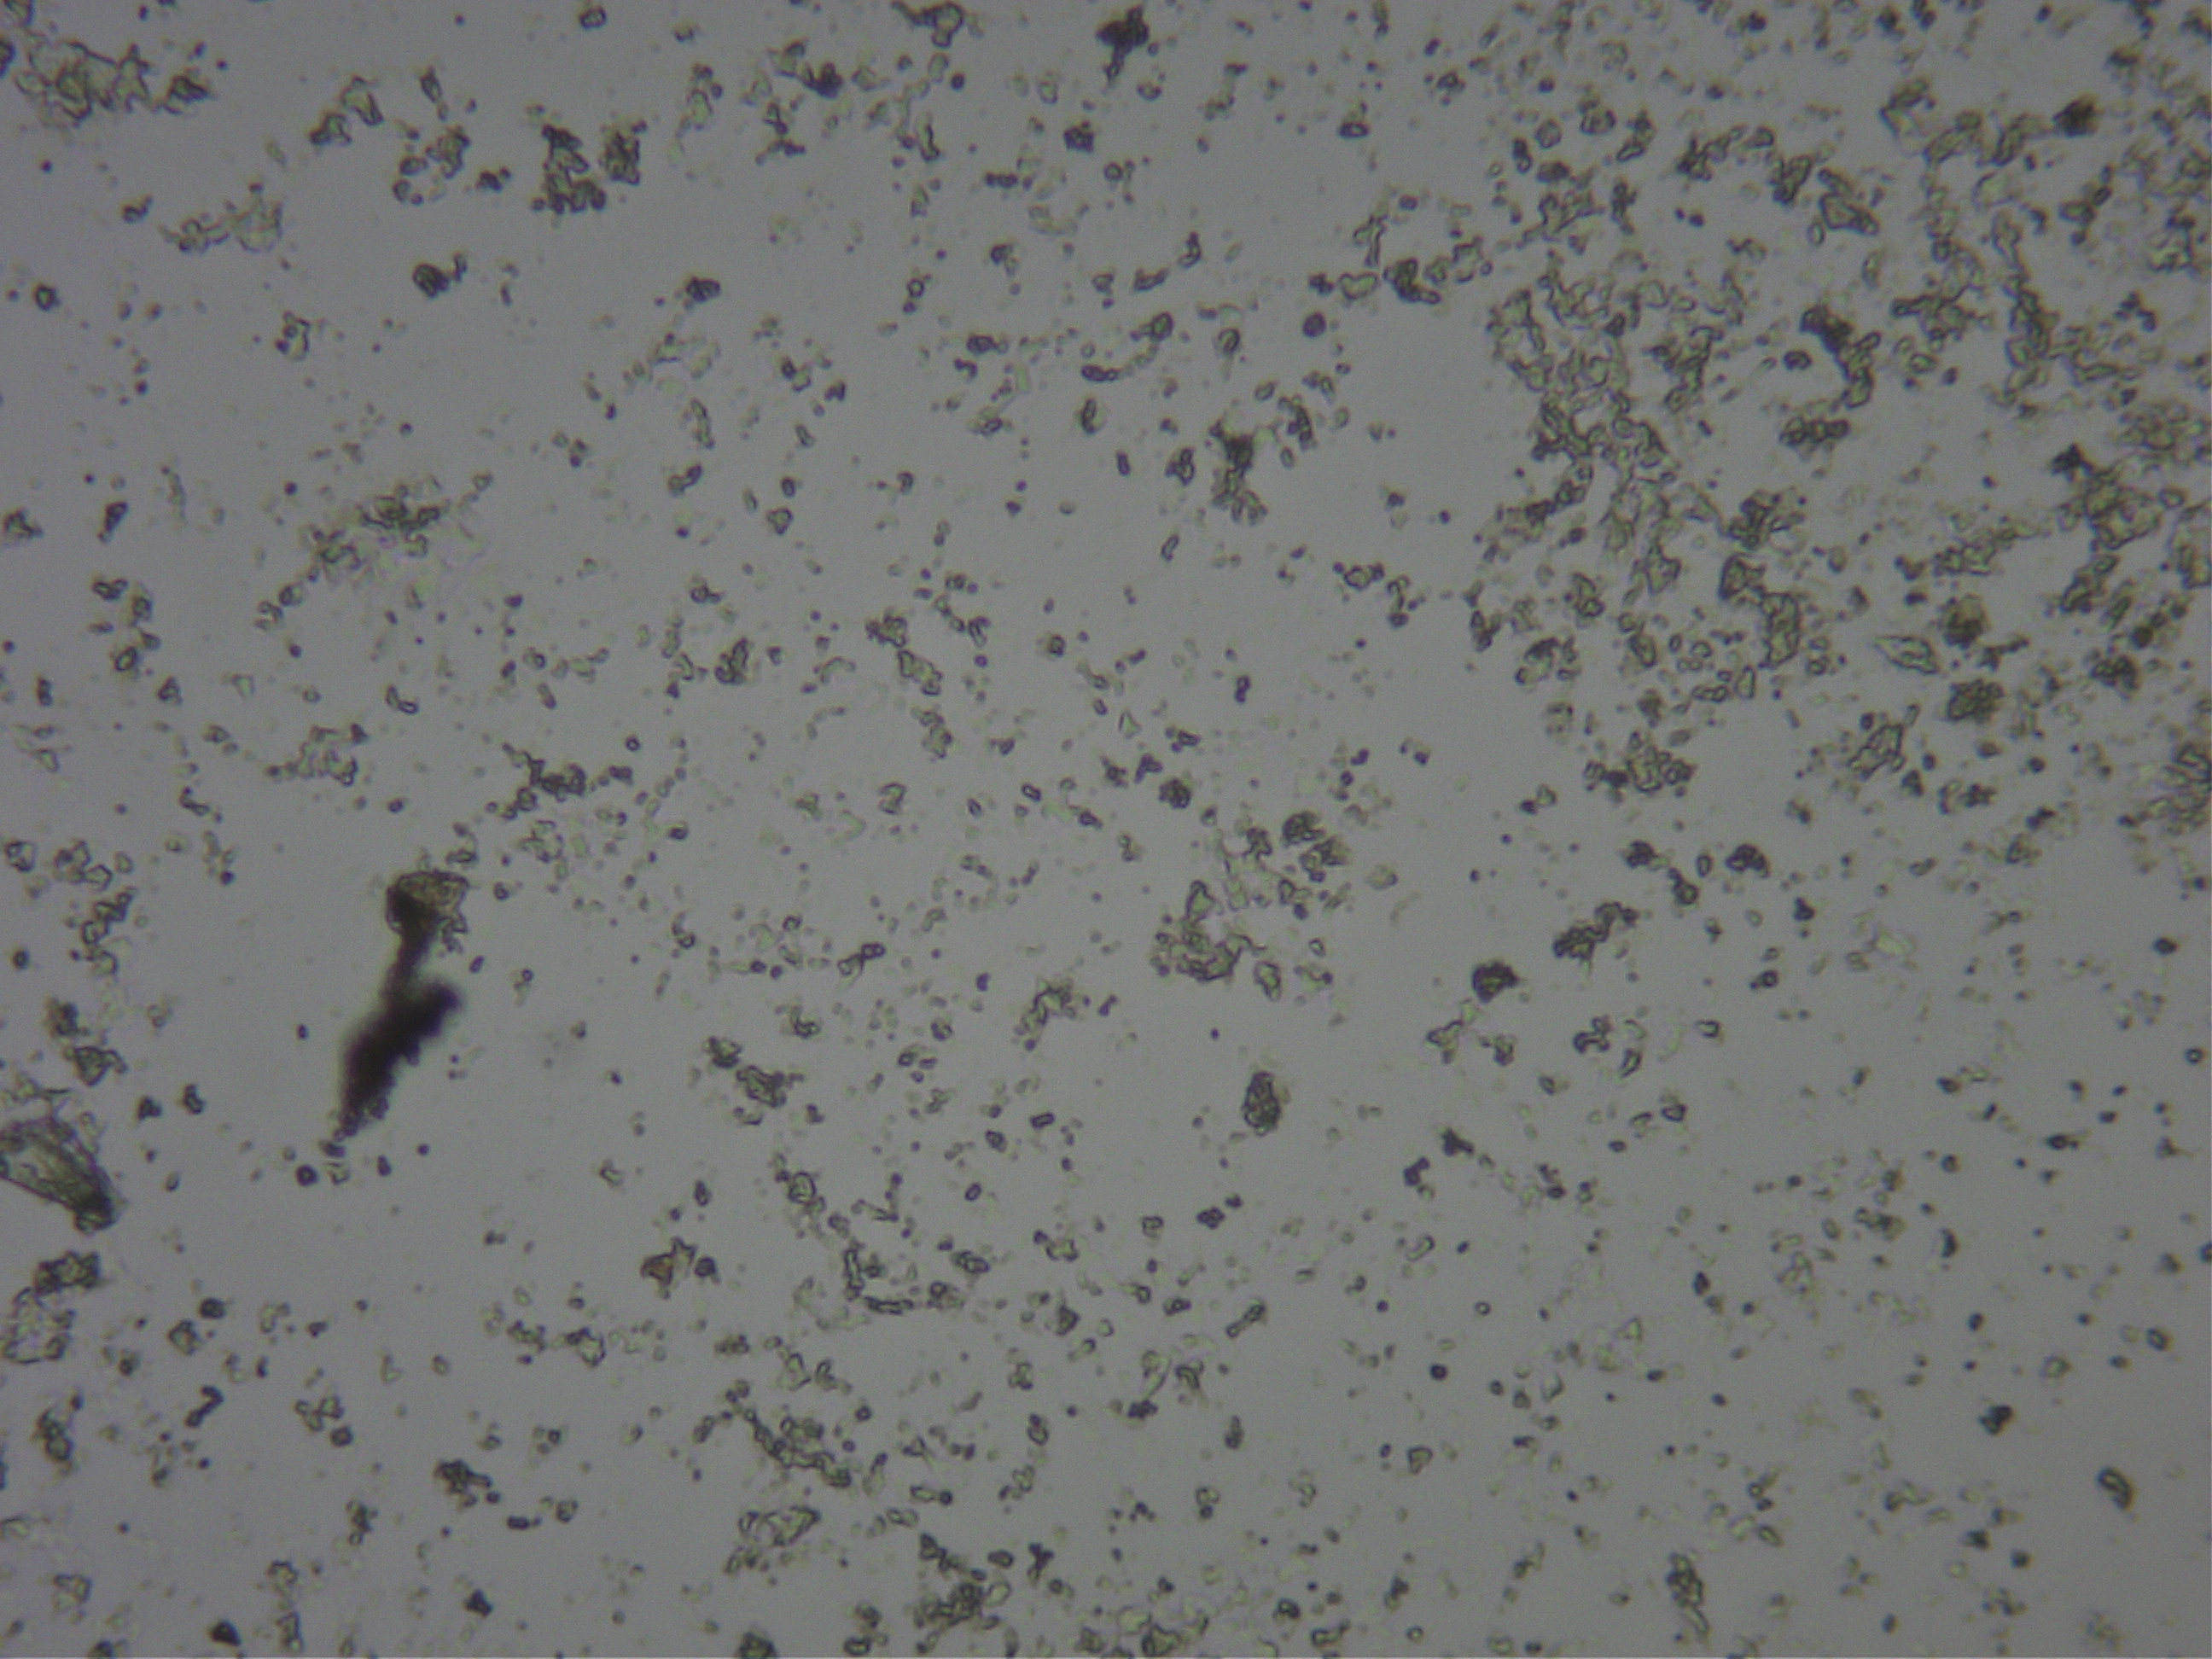
\includegraphics[scale=0.065]{s2.JPG}
    \label{fig:dark}
  \end{subfigure}
  \begin{subfigure}{.4\textwidth}
    \centering
    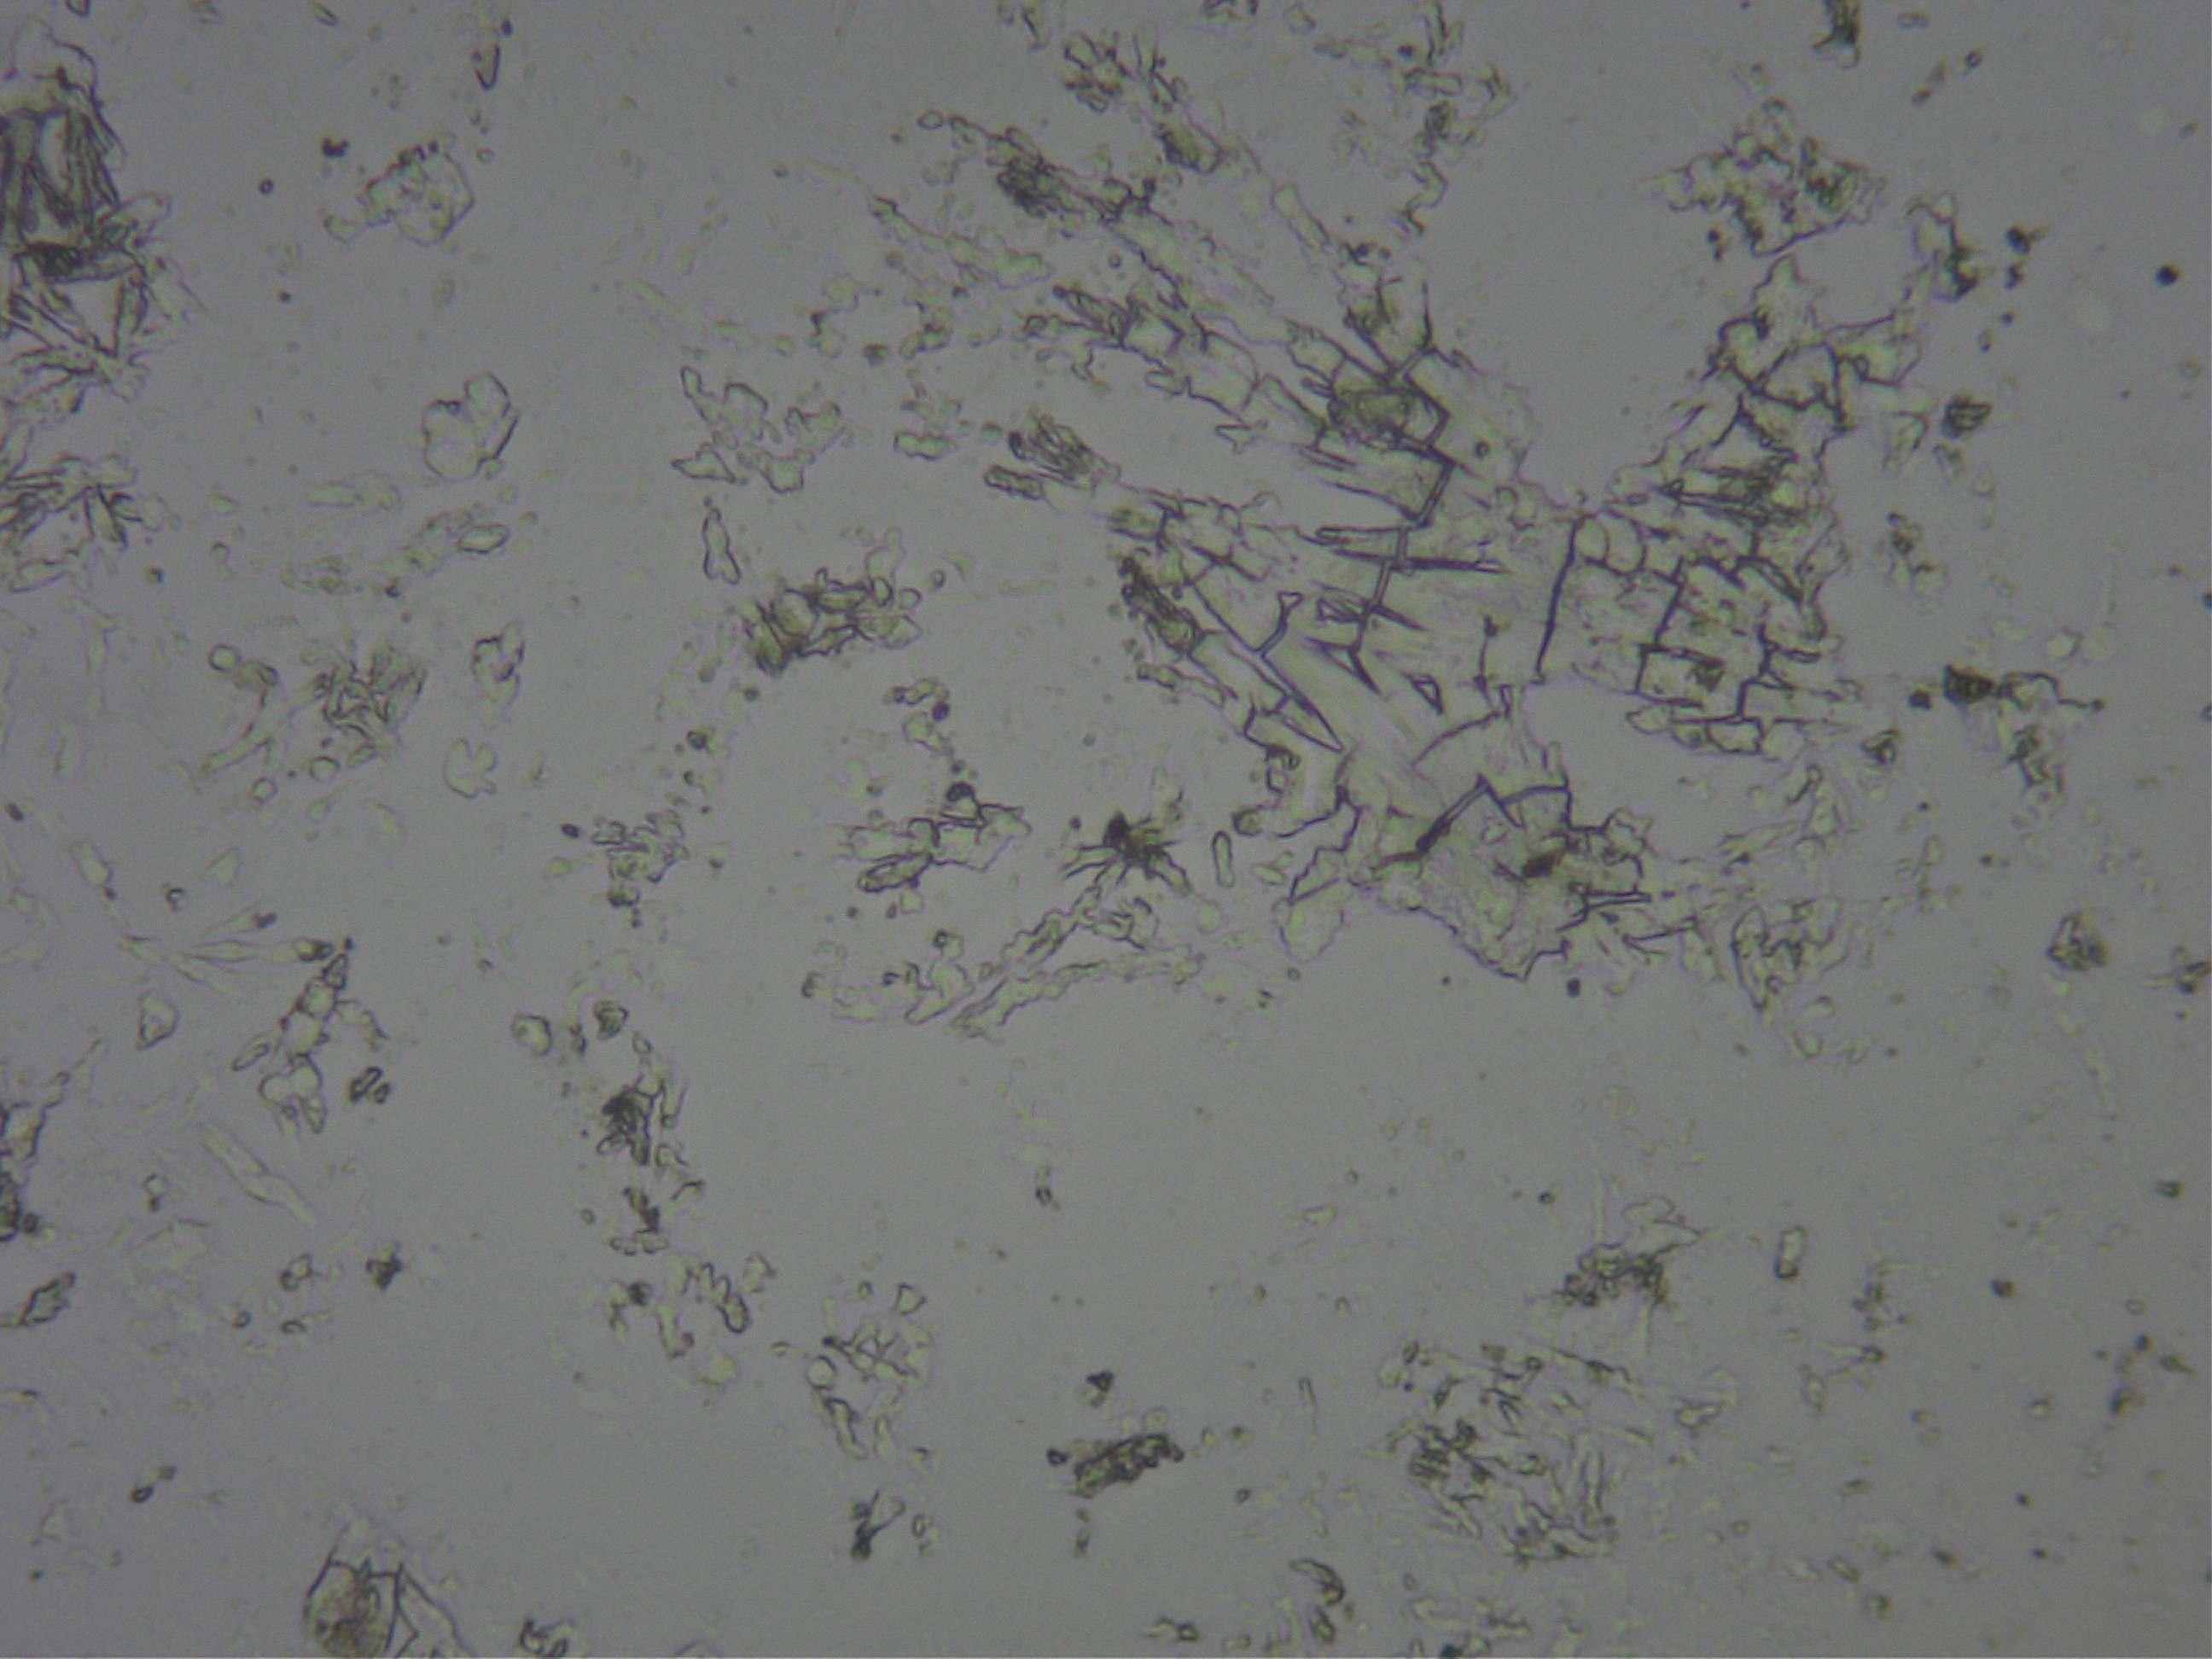
\includegraphics[scale=0.065]{s3.JPG}
    \label{fig:light}
  \end{subfigure}
  \caption[HPO images of thin films]{Microstructure images of a thin film taken under HPO ($40\times$ magnification)}
  \label{fig:hpo}
\end{figure}

It can be seen from the images that the volume covered by the particles in the figures are not ordered (the structures are amorphous).

\section[Comparison of spatial correlations]{Comparison of two point statistics between probe volumes of a thin film}

Discrete microstructure functions were derived from the image data by means of image segmentation using the Yen binary thresholding method.
Upon studying the two point spatial correlations in 360 images, 120 for each type of thin film (S1, S2, S3), it is shown that through principal component analysis that there is no significant difference in the distributions of the particles in the films \cite{gupta15}.
Separated contour plots of the data are shown in Figure \ref{fig:cont}.
The contour plots show the regions where the joint probability of finding zinc oxide in the films at two different sites is the same.
From the figures, it can be observed that the variances of the films are large due to the spacing between the lines and that the shapes of the contours are different.
This suggests that the particles are randomly distributed in the substrate.

\begin{figure}
  \centering
  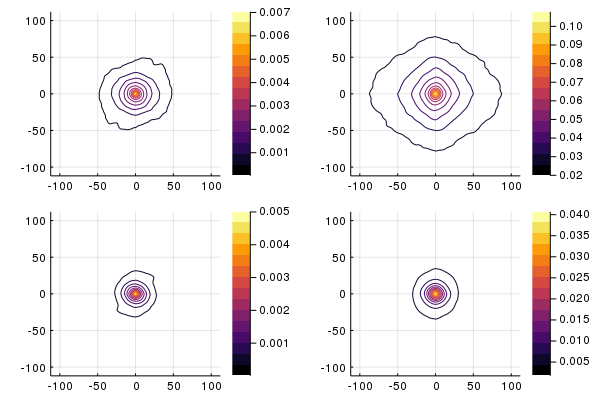
\includegraphics[scale=0.5]{contour.png}
  \caption[Contour plots of spatial correlations]{Contour plots of two point spatial correlations within sections of the same thin film}
  \label{fig:cont}
\end{figure}

\section[Comparison of spatial correlations 2]{Comparison of two point statistics in similar probe volumes of different thin films}

Shown in Figure \ref{fig:pca} are the plots of transformed microstructure function compositions of the particles in the different thin films.
It can be noticed that the plots show that the distributions are random with increasing variance from S1, S2, and S3.
Due to homogeneity of two-point statistics between differentially fabricated thin films, such information cannot be incorporated with existing spatial correlations to make a more representative DMF.

\begin{figure}
  \centering
  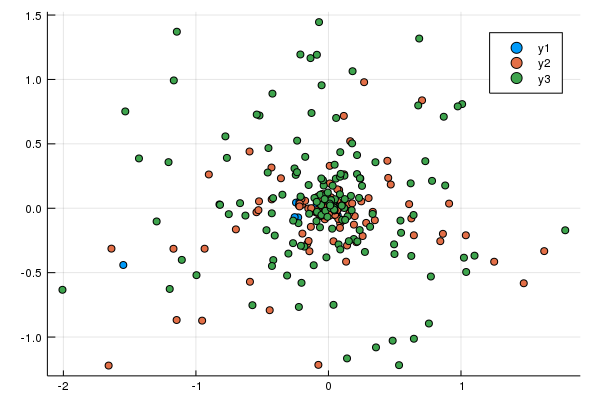
\includegraphics[scale=0.5]{pca.png}
  \caption[Transformed spatial correlations]{Corrected transforms for two-point spatial correlations.}
  \label{fig:pca}
\end{figure}

In a similar study on zinc oxide thin film structure by \citeA{gao08}, they have treated the glass substrate by exposing glass in dilute sulfuric acid.
This led to the adhesion of particulate matter in the aqueous solution.
This process may produce thin films with particulate matter in a non-randomly distributed manner, suggesting that there may be notable differences in two-point spatial correlations.
\citeA{gao08} have prescribed the boiling method coupled witha drying phase between deposition cycles to further improve the crystallinity of the material.

From Figure \ref{fig:cont}, it can be seen that the two-point spatial correlations calculated by the different DMFs have different contour plots.
This is due to the difference in parameters taken into account durin definition (RVE size).
Unfortunately, as was shown through two-point statistics calculations, the structures are random \cite{gupta15}.
This means that no proper modeling methodology can be done due to the homogeneity of the data.

A partial least squares analysis was not performed duw to the homogeneity of two-point statistics as shown through principal component analysis.
